\documentclass[titlepage,11pt,a4paper]{article}
\usepackage[utf8]{inputenc} \usepackage[english]{babel}

% I think these margin options are quite nice
\usepackage[top=1in, bottom=1.25in, left=1.25in,
  right=1.25in]{geometry}

\usepackage{graphicx} \usepackage{float}
\PassOptionsToPackage{hyphens}{url}\usepackage[hidelinks]{hyperref}

\hypersetup{ pdfinfo={ Author={SML}, Title={Developer's Guide},
    Creator={LaTeX} } }

\title{Developer's Guide} \author{SML}


\begin{document}
\maketitle \tableofcontents
\newpage

\section{Introduction}
% Short about our project 
This document describes the different parts of the program for
quadcopters developed on the Access Summer Project, 2015, and before,
in the Smart Mobility Lab, KTH.

% The hardware that we used 
The quadcopters used, and for which this guide is aimed, are the 3DR
IRIS$^+$. As a motion capture system Qualisys was used. The
quadcopters use the Pixhawk autopilot. For changing settings of the
quadcopters the program Mission Planner, version XXX, was used,
\url{http://planner.ardupilot.com/}. Most parts of the code is written
in Python.

% About this guide
This guide provide information about how the program is structured,
Sec.~\ref{sec:architecture}, how ...


\section{Architecture}
\label{sec:architecture}

\begin{figure}[h!]                                                               
  \centering \includegraphics[width=\textwidth]{figures/architecture}
  \caption{The architecture used in ROS. Only main parts and
    connections in shown. X $= 1, 2, 3, \dots$}
  \label{fig:architecture}                                                              
\end{figure}

The program is using ROS, \textit{The Robot Operating System}, to
connect different parts of the program. A basic knowledge of ROS is
assumed. The architecture used in the program is shown in
Fig.~\ref{fig:architecture}. Circles does not correspond to ROS nodes
strictly, but describes the different parts of the
program. Rectangles, however, correspond to ROS topics. ROS packages
are also written in the figure. Arrows with black head corresponds to
publication to a topic, if the arrow points from a circle to a topic,
and subscription to a topic, if the arrow points from a topic to a
circle. Names in the following paragraphs are referring to
Fig.~\ref{fig:architecture}.

The goal of the program is to process commands from the user,
forwarded through the GUI, so that the quadcopter, either in the real
world or in the simulator, acts as the user intends. The GUI can start
different ROS launch files, in turn staring scripts that publishes
points for the quadcopter to follow. These scripts are located in the
trajectory\textunderscore generator package, and for example publishes
points for a line or an arc. Also, the GUI can publish particular
points itself, not using a predefined script. For more information of
the GUI, see Sec.~\ref{sec:gui}. Apart from commands from the user,
information about the quadcopter's location, speed, acceleration,
pitch, roll and yaw is also needed. This is provided by Qualisys,
taken into the ROS framework by the mocap package.

A controller can be applied, since both the target point and the
current point is known. This is done in the controller package. The
current point is processed by the Security Guard. If not the
quadcopter is within certain safety limits, etc., the Lander node is
told to land the quadcopter by the Security Guard. If it is, the
Blender is told to further process the data. The blender got it's name
because it can ``blend'' outputs of different controllers and
collision avoidance. The outputs of the controllers are then
transformed to roll, pitch, throttle and yaw in the Blender. This is
then sent to Mavros on the topic /irisX/mavros/rc/override/ (X $= 1,
2, 3, 4, \dots$) and finally to the quadcopter.


\section{GUI}
\label{sec:gui}

\section{Connecting servos}
\label{sec:servos}
IRIS$^+$ uses the Pixhawk autopilot. On the Pixhawk there are outputs
for servos, shown in Fig.~\ref{fig:pixhawk_outputs}. The outputs are
divided in eight ``main outputs'', MAIN OUT 1-8, and six ``auxiliary
outputs'', AUX OUT 1-6. MAIN OUT 1-4 are occupied by the the four
motors. However, MAIN OUT 1-8 should be avoided for servos anyway
since these update at a rate of 400 Hz by default. AUX OUT 1-6 update
at 50 Hz, which is standard for servos.

\begin{figure}[h!]                                                               
  \centering
  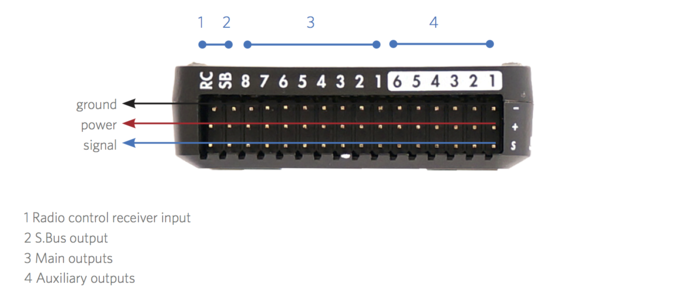
\includegraphics[width=1.0\textwidth]{figures/pixhawk_outputs}
  \caption{Pixhawk outputs for servos. Image from
    \url{http://copter.ardupilot.com/wiki/common-autopilots/common-pixhawk-overview/}.}
  \label{fig:pixhawk_outputs}                                                              
\end{figure}

AUX OUT 5-6 are, by default, set up as relays. The number of AUX OUT
ports set up as servo outputs can be changed in Mission Planner with
the \texttt{BRD\textunderscore PWM\textunderscore COUNT} parameter, in
the way that setting \texttt{BRD\textunderscore PWM\textunderscore
 COUNT} to 6 gives servo output on AUX OUT 1-6.

The IRIS$^+$ transmitter and receiver has eight channels. This is
reflected in the way that a vector of eight components can be sent to
the quad via the topic /irisX/mavros/rc/override/. The first four
components are for roll, pitch, throttle and yaw, leaving the other
four for servos. In addition to that, the different channels needs to
be connected to the different servo outputs on the Pixhawk. This can
be done in the Mission Planner. In Mission Planner, the eight channels
are named RC1-RC8. The different servo ports are named in a similar
way: RC1-RC8 corresponds to MAIN OUT 1-8 and RC9-RC14 corresponds to
AUX OUT 1-6. Unfortunately, in the current version of Mission Planner,
there is no general way of connecting channel RCX to RCY, X $= 1 \dots
8$, Y = $= 1 \dots 14$. If three or less servos are needed, the built
in settings for a camera gimbal can be used.\footnote{Which signals to
be sent to which servo output are controlled by the parameter
\texttt{RCX\textunderscore FUNCTION}, X $= 1 \dots 14$, in Mission
Planner. For these parameters, there is an option called
\texttt{Passthrough}, passing channel X to output X, but since there
are eight channels, only MAIN OUT 1-8 can be reached by this option,
not AUX OUT 1-6.}

The Pixhawk does not provide power to the servos itself, so these must
be powered in other ways. A BEC or ESC, providing 5 V, can be used,
for example. It can be connected to the servo outputs on the Pixhawk
or to the servo directly. By default, the ground pins are connected to
the ground of the battery, by a wire to MAIN OUT 1 ground pin. Also,
on the bottom of the IRIS$^+$ there are a black cable connected to AUX
OUT 6 ground pin and a white cable connected to AUX OUT 1 signal
pin. In addition to this, there is a red power cable and another black
ground wire connected to the battery of the IRIS$^+$, providing 12
V. So, if the voltage is lowered to around 5 V this can be used. So if
only one servo is needed, the quadcopter does not even needs to be
opened!

For additional tips and tricks, see
\url{http://copter.ardupilot.com/wiki/common-optional-hardware/common-servo/}
and \url{https://learn.adafruit.com/quadcopter-spray-can-mod/}. A
wiring diagram for the Pixhawk can be found in
\url{http://copter.ardupilot.com/wiki/advanced-pixhawk-quadcopter-wiring-chart/}.

\end{document}
